
%(BEGIN_QUESTION)
% Copyright 2015, Tony R. Kuphaldt, released under the Creative Commons Attribution License (v 1.0)
% This means you may do almost anything with this work of mine, so long as you give me proper credit

Følgende diagrammer dokumenterer overstrømsvernsystemet for en feeder som forsyner en industriell last med trefaset AC-effekt:

$$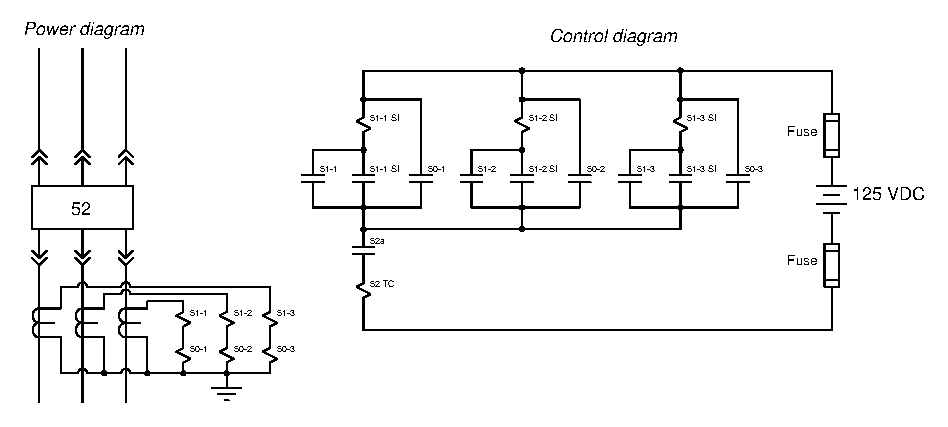
\includegraphics[width=15.5cm]{i01279x01.eps}$$

Anta at effektbryteren (52) en dag løser ut uten åpenbar grunn. Ingen av de fargerike «target»-flaggene på det elektromekaniske vernereléet er synlige, slik man normalt forventer etter en relay-utløsning. Vurder sannsynligheten for hver spesifiserte feil i dette systemet. Betrakt hver feil én om gangen (dvs. ingen samtidige feil), og avgjør om hver feil alene kan forklare {\it alle} målinger og symptomer i denne kretsen.

% No blank lines allowed between lines of an \halign structure!
% I use comments (%) instead, so that TeX doesn't choke.

$$\vbox{\offinterlineskip
\halign{\strut
\vrule \quad\hfil # \ \hfil & 
\vrule \quad\hfil # \ \hfil & 
\vrule \quad\hfil # \ \hfil \vrule \cr
\noalign{\hrule}
%
% First row
{\bf Feil} & {\bf Mulig} & {\bf Umulig} \cr
%
\noalign{\hrule}
%
% Another row
Død DC-forsyning i stasjonen &  &  \cr
%
\noalign{\hrule}
%
% Another row
52/TC-spole feilet kortsluttet &  &  \cr
%
\noalign{\hrule}
%
% Another row
51-3/SI-spole feilet kortsluttet &  &  \cr
%
\noalign{\hrule}
%
% Another row
50-1-kontakt feilet åpen &  &  \cr
%
\noalign{\hrule}
%
% Another row
50-1-kontakt feilet kortsluttet &  &  \cr
%
\noalign{\hrule}
%
% Another row
50-2-spole feilet kortsluttet &  &  \cr
%
\noalign{\hrule}
%
% Another row
50-2-spole feilet åpen &  &  \cr
%
\noalign{\hrule}
} % End of \halign 
}$$ % End of \vbox

Angi også hvilken side av 52-effektbryteren som bør være «line» (forsyning) og hvilken side som bør være «load» for at 50/51-reléet skal gi maksimal beskyttelse i dette systemet.

\vfil 

\underbar{file i01279}
\eject
%(END_QUESTION)





%(BEGIN_ANSWER)

Dette er et vurdert spørsmål -- ingen svar eller hint er gitt!
 
%(END_ANSWER)





%(BEGIN_NOTES)

% No blank lines allowed between lines of an \halign structure!
% I use comments (%) instead, so that TeX doesn't choke.

$$\vbox{\offinterlineskip
\halign{\strut
\vrule \quad\hfil # \ \hfil & 
\vrule \quad\hfil # \ \hfil & 
\vrule \quad\hfil # \ \hfil \vrule \cr
\noalign{\hrule}
%
% First row
{\bf Feil} & {\bf Mulig} & {\bf Umulig} \cr
%
\noalign{\hrule}
%
% Another row
Død DC-forsyning i stasjonen &  & $\surd$ \cr
%
\noalign{\hrule}
%
% Another row
52/TC-spole feilet kortsluttet &  & $\surd$ \cr
%
\noalign{\hrule}
%
% Another row
51-3/SI-spole feilet kortsluttet &  & $\surd$ \cr
%
\noalign{\hrule}
%
% Another row
50-1-kontakt feilet åpen &  & $\surd$ \cr
%
\noalign{\hrule}
%
% Another row
50-1-kontakt feilet kortsluttet & $\surd$ &  \cr
%
\noalign{\hrule}
%
% Another row
50-2-spole feilet kortsluttet &  & $\surd$ \cr
%
\noalign{\hrule}
%
% Another row
50-2-spole feilet åpen &  & $\surd$ \cr
%
\noalign{\hrule}
} % End of \halign 
}$$ % End of \vbox

For maksimal beskyttelse bør reléets vernesone omfatte effektbryteren. Dette betyr at nedre side skal være line og øvre side skal være load. Da vil reléet (med CT-ene på bryterens line-side) oppdage overstrøm også ved intern feil i bryteren og løse den ut.

%INDEX% Electric power systems: protective relays (time-overcurrent)
%INDEX% Protective relay: instantaneous overcurrent (50)
%INDEX% Protective relay: time-overcurrent (51)

%(END_NOTES)

